\documentclass[10pt,UTF8]{ctexart}


\usepackage[margin=2cm,a4paper]{geometry}
%\usepackage[left=0.75in,top=0.6in,right=0.75in,bottom=1.0in,a4paper]{geometry}

\setmainfont{Caladea}
%% 也可以選用其它字庫:
% \setCJKmainfont[%
%   ItalicFont=AR PL KaitiM GB,
%   BoldFont=Noto Sans CJK SC,
% ]{Noto Serif CJK SC}
% \setCJKsansfont{Noto Sans CJK SC}
% \renewcommand{\kaishu}{\CJKfontspec{AR PL KaitiM GB}}

% 繁體中文
\setCJKmainfont[Path=fonts/ ]{NotoSansTC-Medium.otf}

\usepackage{minted}
\usepackage[breaklinks]{hyperref}

% Picture
% 導言區的此三行無變化
\usepackage{graphicx}
\usepackage{float} 
\usepackage{subfigure}
% 以下是新增的自定義格式更改
\usepackage[]{caption2} %新增調用的宏包
\renewcommand{\figurename}{Fig.} %重定義編號前綴詞
\renewcommand{\captionlabeldelim}{.~} %重定義分隔符
 %\roman 是羅馬數字編號,\alph是默認的字母編號,\arabic是阿拉伯數字編號,可按需替換下一行的相應位置
\renewcommand{\thesubfigure}{(\roman{subfigure})}%此外,還可設置圖編號顯示格式,加括號或者不加括號
\makeatletter \renewcommand{\@thesubfigure}{\thesubfigure \space}%子圖編號與名稱的間隔設置
\renewcommand{\p@subfigure}{} \makeatother

% Math
\usepackage {mathtools}
\usepackage{amssymb}

% Code
\usepackage{listings}
\usepackage{xcolor}
\lstset{
    % backgroundcolor=\color{red!50!green!50!blue!50},
    % 程式碼塊背景色為淺灰色
    rulesepcolor= \color{gray}, % 程式碼塊邊框顏色
    breaklines=true,  % 程式碼過長則換行
    numbers=left, % 行號在左側顯示
    numberstyle= \small,% 行號字型
    % eywordstyle= \color{red,% 關鍵字顏色
    commentstyle=\color{gray}, % 註釋顏色
    frame=shadowbox % 用方框框住程式碼塊
    }

\usepackage{hyperref}

\title{數字媒體軟件與系統開發}
\author{干皓丞,2101212850, 信息工程學院}

\begin{document}
\maketitle


\section{作業目標與章節摘要}

FFMGEG 下載,並說明 output\_example 。

\begin{figure}[H]
\centering 
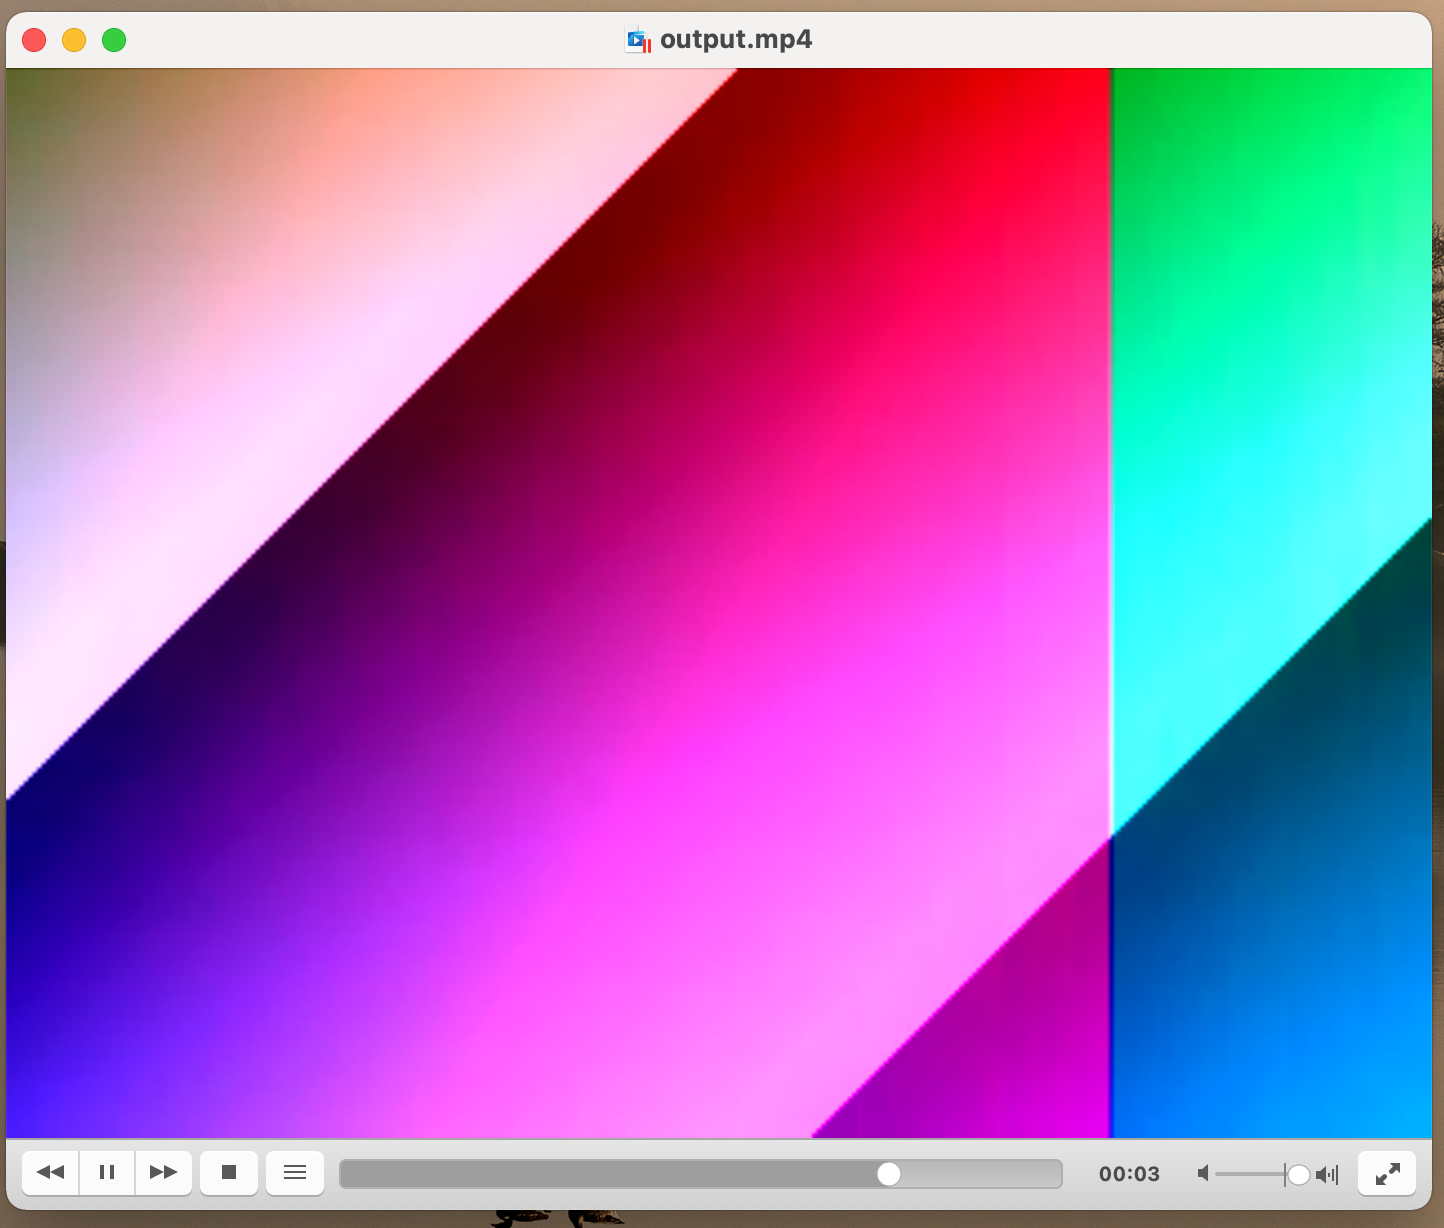
\includegraphics[width=0.90\textwidth]{m1.png} 
\caption{最後測試結果}
\label{Test}
\end{figure}

\section{文章與作業狀況}

作業可以從 GitHub 下的 kancheng/kan-cs-report-in-2022 專案找到,作業程式碼與文件目錄為 kan-cs-report-in-2022/DMSASD/ffmpeg。實際執行的環境與實驗設備為 Google 的 Colab 、MacBook Pro (Retina, 15-inch, Mid 2014) 、 Acer Aspire R7 與 HP Victus (Nvidia GeForce RTX 3060)。

https://github.com/kancheng/kan-cs-report-in-2022/tree/main/DMSASD/ffmpeg

\section{作業內容概述}

此作業分為二大部分,第一部分說明前置準備與分析專案,第二部分則描述 output-example 原始碼與測試該過程,最後補充 /doc/example/muxing.c。

1. 前置準備與分析專案

2. output-example 原始碼與測試該過程

3. /doc/example/muxing.c。

\begin{figure}[H]
\centering 
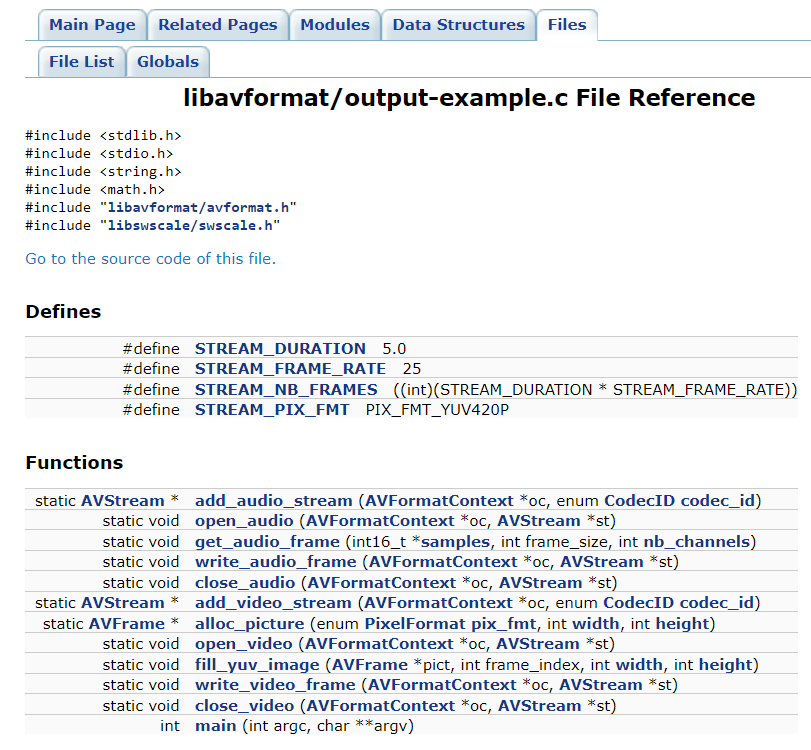
\includegraphics[width=0.50\textwidth]{f1.png} 
\caption{官方文件}
\label{Test}
\end{figure}

\section{前置準備與分析專案}

其官方文件、原始碼檔案與相關連結如下 :

1. https://github.com/FFmpeg/FFmpeg

2. https://www.ffmpeg.org/download.html

3. https://ffmpeg.org/doxygen/0.6/output-example\_8c.html

4. https://ffmpeg.org/doxygen/0.6/output-example\_8c-source.html

5. https://libav.org/documentation/doxygen/master/output\_8c-example.html

6. https://ffmpeg.org/doxygen/trunk/output-example\_8c.html

7. https://ffmpeg.org/doxygen/trunk/output-example\_8c-source.html

8. https://ffmpeg.org/doxygen/trunk/avformat\_8h-source.html

9. https://ffmpeg.org/doxygen/trunk/swscale\_8h-source.html

10. https://ffmpeg.org/doxygen/trunk/mathematics\_8h\_source.html

\subsection{Cloc 分析 FFMPEG}

將下載來的原始碼進行 cloc 指令與結果分析

\begin{lstlisting}[language={python}]
cloc .
\end{lstlisting}

\begin{lstlisting}[language={python}]
(base) PS D:\FFmpeg-n3.0\ffmpeg-raw> cloc .
    7698 text files.
    4341 unique files.
    3359 files ignored.

github.com/AlDanial/cloc v 1.92  T=92.26 s (47.1 files/s, 18264.0 lines/s)
-----------------------------------------------------------------------------------
Language                         files          blank        comment           code
-----------------------------------------------------------------------------------
C                                 2884         161056         107146        1068012
C/C++ Header                      1034          17405          57010         121608
Assembly                           281          11238          12309         100291
Bourne Shell                        22            936            459           8150
make                                40            319             86           4370
C++                                  3            343            143           2206
Objective-C                          5            427            214           2092
CUDA                                 5            259            121           1399
OpenCL                              13            273            359           1349
Perl                                 7            256            349           1050
Markdown                             7            204              0            868
Python                               6            119             97            577
XML                                  9              4              0            432
XSD                                  1             45              4            337
Windows Resource File                8             24            176            240
Metal                                1             34             42            202
CSS                                  3             31             22            140
Verilog-SystemVerilog                8              0              0             56
awk                                  1              6              5             53
Ruby                                 1              9              0             52
HTML                                 1              5              4             44
YAML                                 1              0              0             30
-----------------------------------------------------------------------------------
SUM:                              4341         192993         178546        1313558
-----------------------------------------------------------------------------------
(base) PS D:\FFmpeg-n3.0\ffmpeg-raw>
\end{lstlisting}

\subsection{Mac 編譯 FFMPEG}

嘗試用內部的 configure 進行編譯。

\begin{lstlisting}[language={python}]
./configure --disable-x86asm
ffmpeg
\end{lstlisting}

當然不用編譯,也可以使用 brew 等工具安裝現有編譯好的 FFMPEG。

\begin{figure}[H]
\centering 
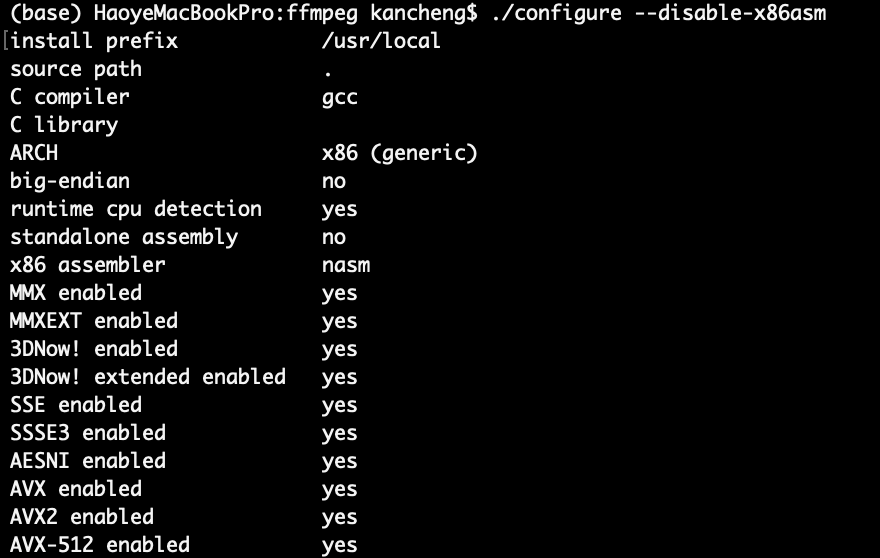
\includegraphics[width=0.80\textwidth]{r1.png} 
\caption{編譯}
\label{Test}
\end{figure}

\begin{figure}[H]
\centering 
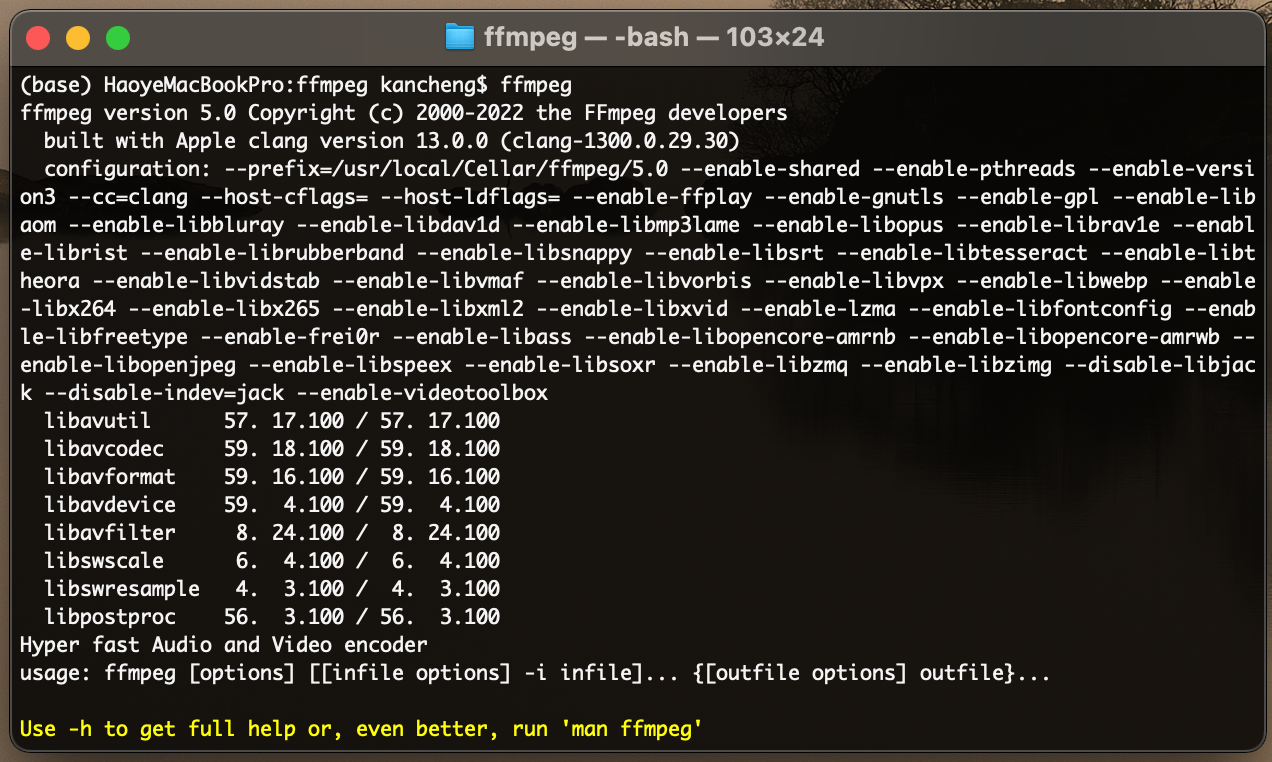
\includegraphics[width=0.80\textwidth]{r2.png} 
\caption{編譯成功}
\label{Test}
\end{figure}

\subsection{output-example.c 版本}

已知社群中文素材所找的內容,其實時間大多為 2010 左右,而該範例原始碼於0.6 還可以找到,但在 0.7 版此檔案就已經被拔掉,其大的版本可以在 v0.6.1 中下載。

從 GitHub 的版本號中可以看到是由 Michael Niedermayer 所提交的合併更動時消失。在此可以用指令將下載來的 FFMPEG 匯出 Git Commit 紀錄,來追專案的變化

將所有 Log 紀錄用指令輸出至一個 txt 檔案中。

\begin{lstlisting}[language={python}]
git log > log.txt
\end{lstlisting}

接下來發現 Michael Niedermayer ,FFMPEG 的專案開發者的相關批改,也就是在這個合併後,該檔案就沒再出現了。

\begin{lstlisting}[language={python}]
commit fbe02459dc4f3c8f4d758c1a90ed8e35a800f3b9
Merge: 9a1963fbb8 b4675d0fbf
Author: Michael Niedermayer <michael@niedermayer.cc>
Date:   Mon Jul 16 01:32:52 2012 +0200

    Merge remote-tracking branch 'qatar/master'
    
    * qatar/master:
      configure: Check for CommandLineToArgvW
      vc1dec: Do not use random pred_flag if motion vector data is skipped
      vp8: Enclose pthread function calls in ifdefs
      snow: refactor code to work around a compiler bug in MSVC.
      vp8: Include the thread headers before using the pthread types
      configure: Check for getaddrinfo in ws2tcpip.h, too
      vp8: implement sliced threading
      vp8: move data from VP8Context->VP8Macroblock
      vp8: refactor decoding a single mb_row
      doc: update api changes with the right commit hashes
      mem: introduce av_malloc_array and av_mallocz_array
    
    Conflicts:
            configure
            doc/APIchanges
            libavcodec/vp8.c
            libavutil/mem.h
            libavutil/version.h
    
    Merged-by: Michael Niedermayer <michaelni@gmx.at>
\end{lstlisting}

為了確定該檔案是否有可能只是改名,過者遷移路徑,在此用另外一個指令繼續。

Git 追檔案更動

\begin{lstlisting}[language={python}]
git log --full-history -- libavformat/output-example.c
\end{lstlisting}

最後發現被搬移至此 doc/examples/output.c ,更後面就沒有該範例的存在。

\begin{lstlisting}[language={python}]
libavformat/output-example.c → doc/examples/output.c
\end{lstlisting}

其 Log 的顯示於此。

\begin{lstlisting}[language={python}]
commit ab81f24ad43bddf77ddd25cba86780c1c884996c
Author: Diego Biurrun <diego@biurrun.de>
Date:   Sat Nov 2 17:05:28 2013 +0100

    build: Integrate multilibrary examples into the build system

    This includes moving libavformat/output-example to doc/examples/output.
\end{lstlisting}

\begin{figure}[H]
\centering 
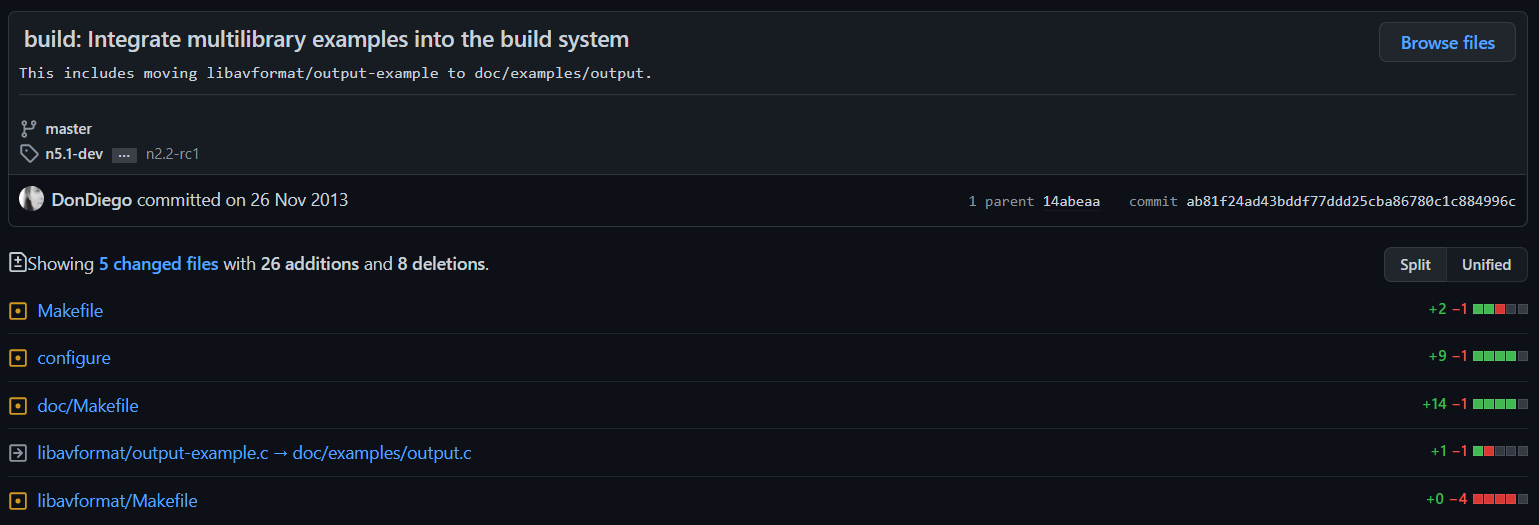
\includegraphics[width=0.80\textwidth]{g1.png} 
\caption{GitHub 紀錄}
\label{Test}
\end{figure}

Git Commit 滾動指令

\begin{lstlisting}[language={python}]
git reset --hard HEAD^
git reset --hard [COMMIT]
\end{lstlisting}

綜上所述,目前遇到有兩個版本,一個是 doc/examples/output.c 最後版本,一個是 libavformat/output-example.c 在最後 v0.6 的版本。在此用 vim 進行對比。

\begin{lstlisting}[language={python}]
vim -d output.c output-example.c
\end{lstlisting}

\begin{figure}[H]
\centering 
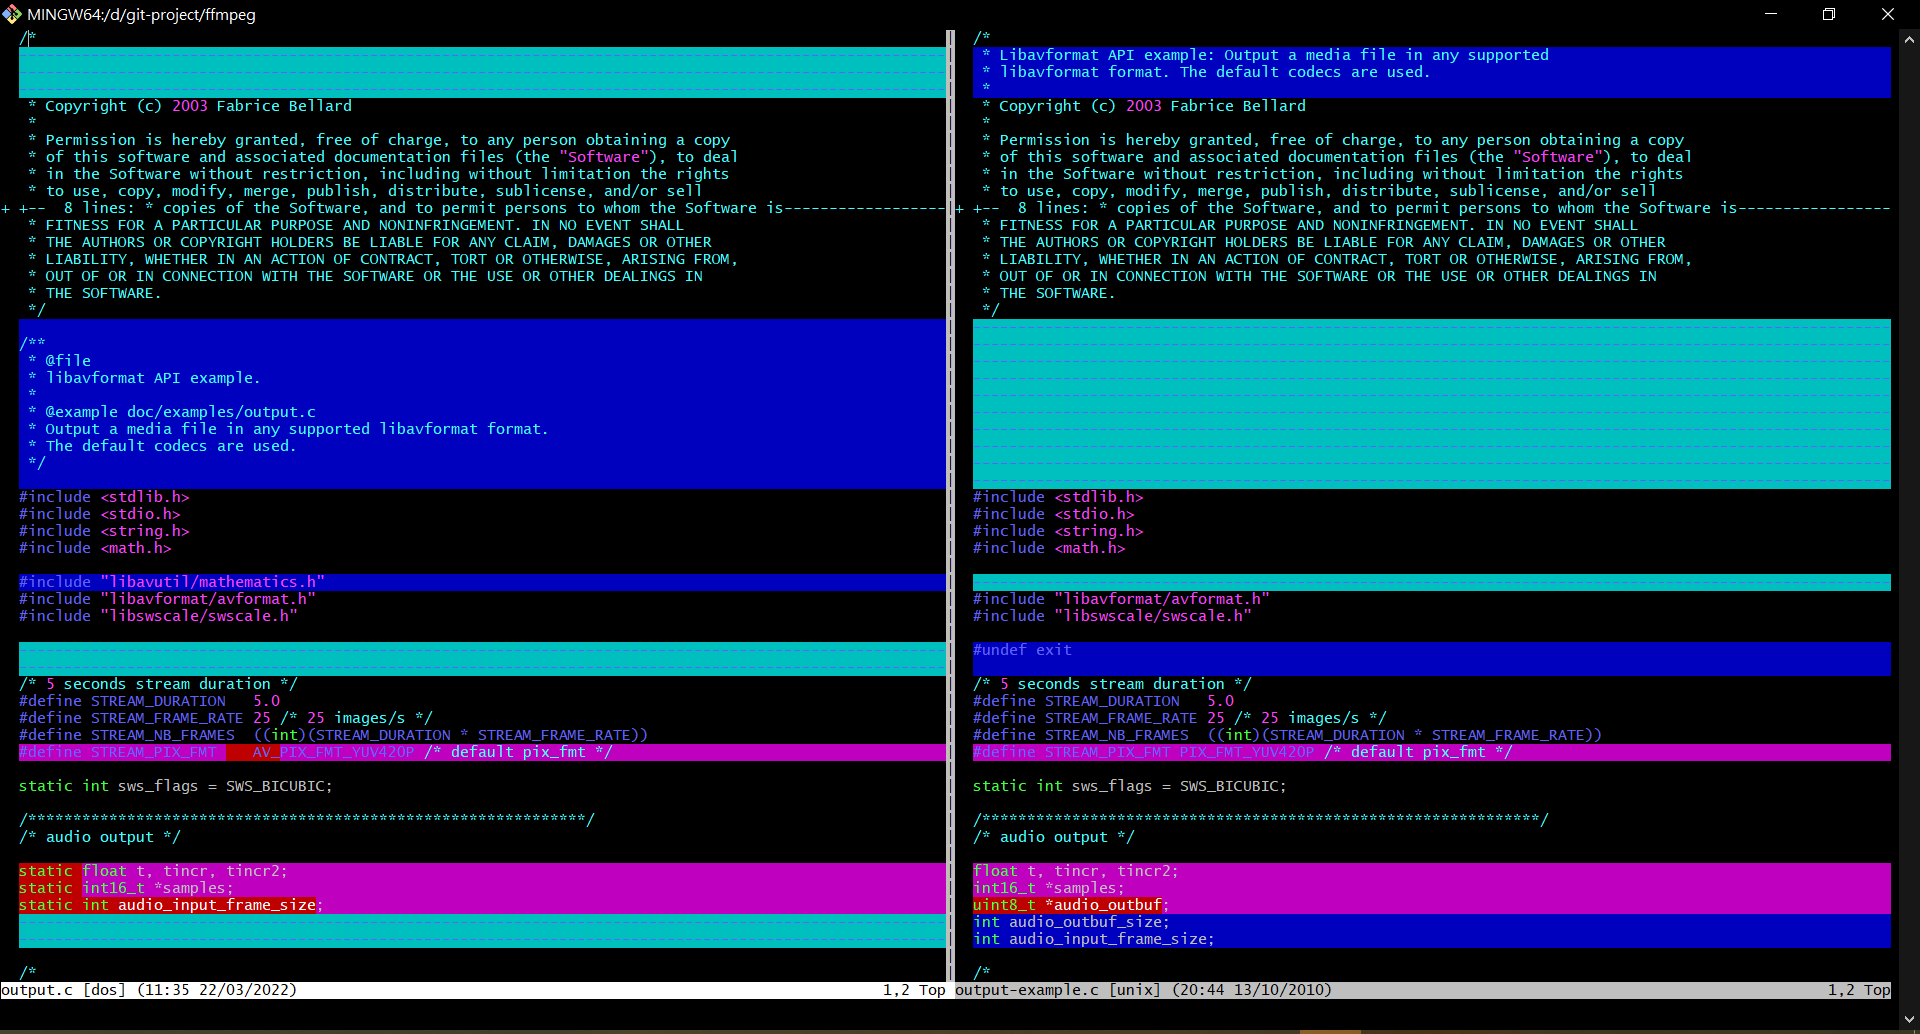
\includegraphics[width=0.80\textwidth]{v1.png} 
\caption{Vim 行數對比}
\label{Test}
\end{figure}

從上面可以看到 doc/examples/output.c 相對 libavformat/output-example.c 多了不少更進,在此,本作業用 doc/examples/output.c 版本進行分析。

\section{output-example}

\subsection{output-example 作業項目}

在此本作業在此針對  doc/examples/output.c 整理成一份檔名為 output-zh-read.c 的中文註解說明版本如下。而後分析都根據官方文件與專案程式碼。

https://github.com/kancheng/kan-cs-report-in-2022/blob/main/DMSASD/ffmpeg/output-zh-read.c

\subsection{output-example 源代碼說明}

該程式碼開頭為給使用者版權宣告註解與先前從 libavformat API example 遷移過來的說明。

\begin{lstlisting}[language={python}]
/*
 * Copyright (c) 2003 Fabrice Bellard
 *
 * Permission is hereby granted, free of charge, to any person obtaining a copy
 * of this software and associated documentation files (the "Software"), to deal
 * in the Software without restriction, including without limitation the rights
 * to use, copy, modify, merge, publish, distribute, sublicense, and/or sell
 * copies of the Software, and to permit persons to whom the Software is
 * furnished to do so, subject to the following conditions:
 *
 * The above copyright notice and this permission notice shall be included in
 * all copies or substantial portions of the Software.
 *
 * THE SOFTWARE IS PROVIDED "AS IS", WITHOUT WARRANTY OF ANY KIND, EXPRESS OR
 * IMPLIED, INCLUDING BUT NOT LIMITED TO THE WARRANTIES OF MERCHANTABILITY,
 * FITNESS FOR A PARTICULAR PURPOSE AND NONINFRINGEMENT. IN NO EVENT SHALL
 * THE AUTHORS OR COPYRIGHT HOLDERS BE LIABLE FOR ANY CLAIM, DAMAGES OR OTHER
 * LIABILITY, WHETHER IN AN ACTION OF CONTRACT, TORT OR OTHERWISE, ARISING FROM,
 * OUT OF OR IN CONNECTION WITH THE SOFTWARE OR THE USE OR OTHER DEALINGS IN
 * THE SOFTWARE.
 */

/**
 * @file
 * libavformat API example.
 *
 * @example doc/examples/output.c
 * Output a media file in any supported libavformat format.
 * The default codecs are used.
 */
\end{lstlisting}

再來就是該程式碼的 C 語言套件庫,部分包含常用的 stdlib.h 、stdio.h、string.h、math.h。FFMPEG 自身的 Library,當中包含了 mathematics.h 數學處理包,與 AVFormat 有關的 avformat.h。跟比如將 YUV420P 轉換成 YUYV422 會用到的換圖大小 swscale.h。
最後則是該程式會需要的巨集定義與相關的變數宣告

\begin{lstlisting}[language={python}]
// C Library

#include <stdlib.h>
#include <stdio.h>
#include <string.h>
#include <math.h>

// FFMPEG Library
#include "libavutil/mathematics.h"
#include "libavformat/avformat.h"
#include "libswscale/swscale.h"

// 巨集定義
/* 5 seconds stream duration */
#define STREAM_DURATION   5.0
#define STREAM_FRAME_RATE 25 /* 25 images/s */
#define STREAM_NB_FRAMES  ((int)(STREAM_DURATION * STREAM_FRAME_RATE))
#define STREAM_PIX_FMT    AV_PIX_FMT_YUV420P /* default pix_fmt */

static int sws_flags = SWS_BICUBIC;
\end{lstlisting}

AVStream 為負責音源輸出與加入加入音源輸出的函式。當中有個尋找音頻編碼器會判斷,然後放入樣本參數,另外在一些 stream header 進行額外處理。

\begin{lstlisting}[language={python}]
// 音源輸出
static float t, tincr, tincr2;
static int16_t *samples;
static int audio_input_frame_size;

/* 加入音源輸出
 * add an audio output stream
 */
static AVStream *add_audio_stream(AVFormatContext *oc, enum AVCodecID codec_id)
{
    AVCodecContext *c;
    AVStream *st;
    AVCodec *codec;
// 找到音頻編碼器
    /* find the audio encoder */
    codec = avcodec_find_encoder(codec_id);
    if (!codec) {
        fprintf(stderr, "codec not found\n");
        exit(1);
    }

    st = avformat_new_stream(oc, codec);
    if (!st) {
        fprintf(stderr, "Could not alloc stream\n");
        exit(1);
    }

    c = st->codec;

// 放樣本參數
    /* put sample parameters */
    c->sample_fmt  = AV_SAMPLE_FMT_S16;
    c->bit_rate    = 64000;
    c->sample_rate = 44100;
    c->channels    = 2;

// 某些格式希望 stream header 是分開的
    // some formats want stream headers to be separate
    if (oc->oformat->flags & AVFMT_GLOBALHEADER)
        c->flags |= CODEC_FLAG_GLOBAL_HEADER;

    return st;
}
\end{lstlisting}

開啟音源函式部分,該函數會進行初始化。當中會有 以每秒 110 Hz 的速度遞增頻率,M\_PI則是 FFMPEG 的 mathematics.h。

\begin{lstlisting}[language={python}]
static void open_audio(AVFormatContext *oc, AVStream *st)
{
    AVCodecContext *c;

    c = st->codec;

    /* open it */
    if (avcodec_open2(c, NULL, NULL) < 0) {
        fprintf(stderr, "could not open codec\n");
        exit(1);
    }

    /* init signal generator */
    t     = 0;
    tincr = 2 * M_PI * 110.0 / c->sample_rate;
    /* increment frequency by 110 Hz per second */
    tincr2 = 2 * M_PI * 110.0 / c->sample_rate / c->sample_rate;

    if (c->codec->capabilities & CODEC_CAP_VARIABLE_FRAME_SIZE)
        audio_input_frame_size = 10000;
    else
        audio_input_frame_size = c->frame_size;
    samples = av_malloc(audio_input_frame_size *
                        av_get_bytes_per_sample(c->sample_fmt) *
                        c->channels);
}
\end{lstlisting}

get\_audio\_frame 準備“frame\_size”樣本的 16 位虛擬音頻幀和 'nb\_channels' 頻道。

\begin{lstlisting}[language={python}]
static void get_audio_frame(int16_t *samples, int frame_size, int nb_channels)
{
    int j, i, v;
    int16_t *q;

    q = samples;
    for (j = 0; j < frame_size; j++) {
        v = (int)(sin(t) * 10000);
        for (i = 0; i < nb_channels; i++)
            *q++ = v;
        t     += tincr;
        tincr += tincr2;
    }
}
\end{lstlisting}

write\_audio\_frame 則是進行編碼工作,pkt 的數據和大小初始必須為 0,其後將壓縮幀寫入媒體文件。

\begin{lstlisting}[language={python}]
static void write_audio_frame(AVFormatContext *oc, AVStream *st)
{
    AVCodecContext *c;
    AVPacket pkt = { 0 }; // data and size must be 0;
    AVFrame *frame = av_frame_alloc();
    int got_packet;

    av_init_packet(&pkt);
    c = st->codec;

    get_audio_frame(samples, audio_input_frame_size, c->channels);
    frame->nb_samples = audio_input_frame_size;
    avcodec_fill_audio_frame(frame, c->channels, c->sample_fmt,
                             (uint8_t *)samples,
                             audio_input_frame_size *
                             av_get_bytes_per_sample(c->sample_fmt) *
                             c->channels, 1);

    avcodec_encode_audio2(c, &pkt, frame, &got_packet);
    if (!got_packet)
        return;

    pkt.stream_index = st->index;

    /* Write the compressed frame to the media file. */
    if (av_interleaved_write_frame(oc, &pkt) != 0) {
        fprintf(stderr, "Error while writing audio frame\n");
        exit(1);
    }
    avcodec_free_frame(&frame);
}
\end{lstlisting}

close\_audio 為關閉音源。

\begin{lstlisting}[language={python}]
static void close_audio(AVFormatContext *oc, AVStream *st)
{
    avcodec_close(st->codec);

    av_free(samples);
}
\end{lstlisting}

AVStream 部分為影像輸出部分,過程中會先找到影像的 encoder,而後放其參數,且設分辨率必須是二的倍數。而 timebase 這是表示幀時間戳的基本時間單位(以秒為單位)。 對於固定 fps 內容,時基應為 1/幀速率,時間戳增量應等於 1。最後最多每十二幀發射一幀。同時為了需要避免使用某些係數溢出的宏塊。
這不會發生在普通視頻中,它只是在這裡發生,因為色度平面的運動與亮度平面不匹配。另外為了測試添加了 B 幀。

\begin{lstlisting}[language={python}]
static AVFrame *picture, *tmp_picture;
static int frame_count;
static AVStream *add_video_stream(AVFormatContext *oc, enum AVCodecID codec_id)
{
    AVCodecContext *c;
    AVStream *st;
    AVCodec *codec;
    codec = avcodec_find_encoder(codec_id);
    if (!codec) {
        fprintf(stderr, "codec not found\n");
        exit(1);
    }
    st = avformat_new_stream(oc, codec);
    if (!st) {
        fprintf(stderr, "Could not alloc stream\n");
        exit(1);
    }
    c = st->codec;
    c->bit_rate = 400000;
    c->width    = 352;
    c->height   = 288;
    c->time_base.den = STREAM_FRAME_RATE;
    c->time_base.num = 1;
    c->gop_size      = 12;
    c->pix_fmt       = STREAM_PIX_FMT;
    if (c->codec_id == AV_CODEC_ID_MPEG2VIDEO) {
        c->max_b_frames = 2;
    }
    if (c->codec_id == AV_CODEC_ID_MPEG1VIDEO) {
        c->mb_decision = 2;
    }
    if (oc->oformat->flags & AVFMT_GLOBALHEADER)
        c->flags |= CODEC_FLAG_GLOBAL_HEADER;
    return st;
}
\end{lstlisting}

AVFrame 為處理 AVCodecContext 的重要組成部分。

\begin{lstlisting}[language={python}]
static AVFrame *alloc_picture(enum AVPixelFormat pix_fmt, int width, int height)
{
    AVFrame *picture;
    uint8_t *picture_buf;
    int size;

    picture = av_frame_alloc();
    if (!picture)
        return NULL;
    size        = avpicture_get_size(pix_fmt, width, height);
    picture_buf = av_malloc(size);
    if (!picture_buf) {
        av_free(picture);
        return NULL;
    }
    avpicture_fill((AVPicture *)picture, picture_buf,
                   pix_fmt, width, height);
    return picture;
}
\end{lstlisting}

open\_video 為開啟影像函式,當中有一個 codec,同時分配編碼的原始圖片,同時如果輸出格式不是 YUV420P,那麼也需要一張臨時的 YUV420P 圖片。 然後將其轉換為所需的輸出格式。

\begin{lstlisting}[language={python}]
static void open_video(AVFormatContext *oc, AVStream *st)
{
    AVCodecContext *c;
    c = st->codec;
    if (avcodec_open2(c, NULL, NULL) < 0) {
        fprintf(stderr, "could not open codec\n");
        exit(1);
    }
    picture = alloc_picture(c->pix_fmt, c->width, c->height);
    if (!picture) {
        fprintf(stderr, "Could not allocate picture\n");
        exit(1);
    }
    tmp_picture = NULL;
    if (c->pix_fmt != AV_PIX_FMT_YUV420P) {
        tmp_picture = alloc_picture(AV_PIX_FMT_YUV420P, c->width, c->height);
        if (!tmp_picture) {
            fprintf(stderr, "Could not allocate temporary picture\n");
            exit(1);
        }
    }
}
\end{lstlisting}

fill\_yuv\_image 的函式為 dummy image 的處理,當中控制 Y 、Cb、Cr。

\begin{lstlisting}[language={python}]
static void fill_yuv_image(AVFrame *pict, int frame_index,
                           int width, int height)
{
    int x, y, i;
    i = frame_index;
    for (y = 0; y < height; y++)
        for (x = 0; x < width; x++)
            pict->data[0][y * pict->linesize[0] + x] = x + y + i * 3;
    for (y = 0; y < height / 2; y++) {
        for (x = 0; x < width / 2; x++) {
            pict->data[1][y * pict->linesize[1] + x] = 128 + y + i * 2;
            pict->data[2][y * pict->linesize[2] + x] = 64 + x + i * 5;
        }
    }
}

\end{lstlisting}

write\_video\_frame 在此處理影像,不再需要壓縮幀。 如果使用 B 幀,編解碼器有幾幀的延遲,所以我們通過再次傳遞相同的圖片來獲得最後一幀,由於該函式只生成一張 YUV420P 圖片,如果需要會將其轉換為編解碼器像素格式。而後面則是 encode 影像的處理。最後將壓縮幀寫入媒體文件。

\begin{lstlisting}[language={python}]
static void write_video_frame(AVFormatContext *oc, AVStream *st)
{
    int ret;
    AVCodecContext *c;
    static struct SwsContext *img_convert_ctx;

    c = st->codec;

    if (frame_count >= STREAM_NB_FRAMES) {
    } else {
        if (c->pix_fmt != AV_PIX_FMT_YUV420P) {
            if (img_convert_ctx == NULL) {
                img_convert_ctx = sws_getContext(c->width, c->height,
                                                 AV_PIX_FMT_YUV420P,
                                                 c->width, c->height,
                                                 c->pix_fmt,
                                                 sws_flags, NULL, NULL, NULL);
                if (img_convert_ctx == NULL) {
                    fprintf(stderr,
                            "Cannot initialize the conversion context\n");
                    exit(1);
                }
            }
            fill_yuv_image(tmp_picture, frame_count, c->width, c->height);
            sws_scale(img_convert_ctx, tmp_picture->data, tmp_picture->linesize,
                      0, c->height, picture->data, picture->linesize);
        } else {
            fill_yuv_image(picture, frame_count, c->width, c->height);
        }
    }

    if (oc->oformat->flags & AVFMT_RAWPICTURE) {
        AVPacket pkt;
        av_init_packet(&pkt);
        pkt.flags        |= AV_PKT_FLAG_KEY;
        pkt.stream_index  = st->index;
        pkt.data          = (uint8_t *)picture;
        pkt.size          = sizeof(AVPicture);
        ret = av_interleaved_write_frame(oc, &pkt);
    } else {
        AVPacket pkt = { 0 };
        int got_packet;
        av_init_packet(&pkt);
        ret = avcodec_encode_video2(c, &pkt, picture, &got_packet);
        if (!ret && got_packet && pkt.size) {
            if (pkt.pts != AV_NOPTS_VALUE) {
                pkt.pts = av_rescale_q(pkt.pts,
                                       c->time_base, st->time_base);
            }
            if (pkt.dts != AV_NOPTS_VALUE) {
                pkt.dts = av_rescale_q(pkt.dts,
                                       c->time_base, st->time_base);
            }
            pkt.stream_index = st->index;
            ret = av_interleaved_write_frame(oc, &pkt);
        } else {
            ret = 0;
        }
    }
    if (ret != 0) {
        fprintf(stderr, "Error while writing video frame\n");
        exit(1);
    }
    frame_count++;
}
\end{lstlisting}

close\_video 關閉影像函式。

\begin{lstlisting}[language={python}]
static void close_video(AVFormatContext *oc, AVStream *st)
{
    avcodec_close(st->codec);
    av_free(picture->data[0]);
    av_free(picture);
    if (tmp_picture) {
        av_free(tmp_picture->data[0]);
        av_free(tmp_picture);
    }
}
\end{lstlisting}

最後則是 main 函式,已開始會初始化 libavcodec,並註冊所有編解碼器和格式,並且從名稱中自動檢測輸出格式。 默認為 MPEG,而後分配輸出媒體內文,最後使用默認格式編解碼器添加音頻和視頻流並初始化編解碼器。

當現在所有參數都設置好後,則可以打開音頻和視頻編解碼器並分配必要的編碼緩衝區。另外過程中有需要,可打開輸出文件,並寫入 stream header,計算計算當前的音頻和視頻時間,最後寫入交錯的音頻和視頻幀與關閉每一個 codec 跟輸出檔案。

\begin{lstlisting}[language={python}]
int main(int argc, char **argv)
{
    const char *filename;
    AVOutputFormat *fmt;
    AVFormatContext *oc;
    AVStream *audio_st, *video_st;
    double audio_pts, video_pts;
    int i;
    av_register_all();
    if (argc != 2) {
        printf("usage: %s output_file\n"
               "API example program to output a media file with libavformat.\n"
               "The output format is automatically guessed according to the file extension.\n"
               "Raw images can also be output by using '%%d' in the filename\n"
               "\n", argv[0]);
        return 1;
    }

    filename = argv[1];
    fmt = av_guess_format(NULL, filename, NULL);
    if (!fmt) {
        printf("Could not deduce output format from file extension: using MPEG.\n");
        fmt = av_guess_format("mpeg", NULL, NULL);
    }
    if (!fmt) {
        fprintf(stderr, "Could not find suitable output format\n");
        return 1;
    }
    oc = avformat_alloc_context();
    if (!oc) {
        fprintf(stderr, "Memory error\n");
        return 1;
    }
    oc->oformat = fmt;
    snprintf(oc->filename, sizeof(oc->filename), "%s", filename);
    video_st = NULL;
    audio_st = NULL;
    if (fmt->video_codec != AV_CODEC_ID_NONE) {
        video_st = add_video_stream(oc, fmt->video_codec);
    }
    if (fmt->audio_codec != AV_CODEC_ID_NONE) {
        audio_st = add_audio_stream(oc, fmt->audio_codec);
    }
    if (video_st)
        open_video(oc, video_st);
    if (audio_st)
        open_audio(oc, audio_st);

    av_dump_format(oc, 0, filename, 1);
    if (!(fmt->flags & AVFMT_NOFILE)) {
        if (avio_open(&oc->pb, filename, AVIO_FLAG_WRITE) < 0) {
            fprintf(stderr, "Could not open '%s'\n", filename);
            return 1;
        }
    }
    avformat_write_header(oc, NULL);
    for (;;) {
        if (audio_st)
            audio_pts = (double)audio_st->pts.val * audio_st->time_base.num / audio_st->time_base.den;
        else
            audio_pts = 0.0;

        if (video_st)
            video_pts = (double)video_st->pts.val * video_st->time_base.num /
                        video_st->time_base.den;
        else
            video_pts = 0.0;
        if ((!audio_st || audio_pts >= STREAM_DURATION) &&
            (!video_st || video_pts >= STREAM_DURATION))
            break;
        if (!video_st || (video_st && audio_st && audio_pts < video_pts)) {
            write_audio_frame(oc, audio_st);
        } else {
            write_video_frame(oc, video_st);
        }
    }
    av_write_trailer(oc);
    if (video_st)
        close_video(oc, video_st);
    if (audio_st)
        close_audio(oc, audio_st);
    for (i = 0; i < oc->nb_streams; i++) {
        av_freep(&oc->streams[i]->codec);
        av_freep(&oc->streams[i]);
    }
    if (!(fmt->flags & AVFMT_NOFILE))
        avio_close(oc->pb);
    av_free(oc);
    return 0;
}

\end{lstlisting}


\subsection{output-example 測試工作}

在此使用 GCC 進行編譯,並針對 ffmpeg 0.5.13 的版本進行測試。架設過去的 Linux 跟 GCC 按照當時的技術文件進行還原。

\begin{lstlisting}[language={python}]
# 下載早期版本
# wget http://www.ffmpeg.org/releases/ffmpeg-0.5.13.tar.bz2

# 解壓縮
# tar -jxvf ffmpeg-0.5.13.tar.bz2

# vim ffmpeg_configure.sh
./configure \
--prefix=/YOUR_INSTLL_DIRECTORY \
--enable-gpl --enable-nonfree --enable-version3 \
--enable-swscale --enable-avfilter  \
--enable-pthreads
【保存并退出】

\end{lstlisting}

進入目錄用 vim 建立 ffmpeg\_configure.sh ,完成後退出。

\begin{lstlisting}[language={python}]
# vim ffmpeg_configure.sh
\end{lstlisting}

\begin{lstlisting}[language={python}]
./configure \
--prefix=/YOUR_INSTLL_DIRECTORY \
--enable-gpl --enable-nonfree --enable-version3 \
--enable-swscale --enable-avfilter  \
--enable-pthreads
\end{lstlisting}

改變權限後用 make 

\begin{lstlisting}[language={python}]
# chmod +x ffmpeg_configure.sh
# ./ffmpeg_configure.sh
# make
# make install
\end{lstlisting}

將安裝目錄“”下的 

YOUR\_INSTLL\_DIRECTORY/include
YOUR\_INSTLL\_DIRECTORY/lib

打包,就可以生成一個開發用的SDK

\begin{lstlisting}[language={python}]
# tar -czvf YOUR_INSTLL_DIRECTORY/ ffmpeg_sdk.tar.gz
\end{lstlisting}

引入後編譯,解决:

\begin{lstlisting}[language={python}]
# gcc output_example.c -o output_example 
-I/opt/ffmpeg/sourcecode/ffmpeg-0.5.13.install/include 
-L/opt/ffmpeg/sourcecode/ffmpeg-0.5.13.install/lib  
-lavformat -lavdevice -lavcodec  -lavutil -lavfilter 
-pthread -ldl -lswscale -lbz2 -lasound  -lz -lm
\end{lstlisting}

運行

\begin{lstlisting}[language={python}]
# ./output_example xxx.flv
\end{lstlisting}

\begin{figure}[H]
\centering 

\includegraphics[width=0.50\textwidth]{tem1.png} 
\caption{output-example 測試結果}
\label{Test}
\end{figure}

\section{muxing.c 測試工作}

後來經過調研才發現類似的 Code 於此, 其測試內容於之前雷同,但是這回使用 Mac。

\begin{figure}[H]
\centering 
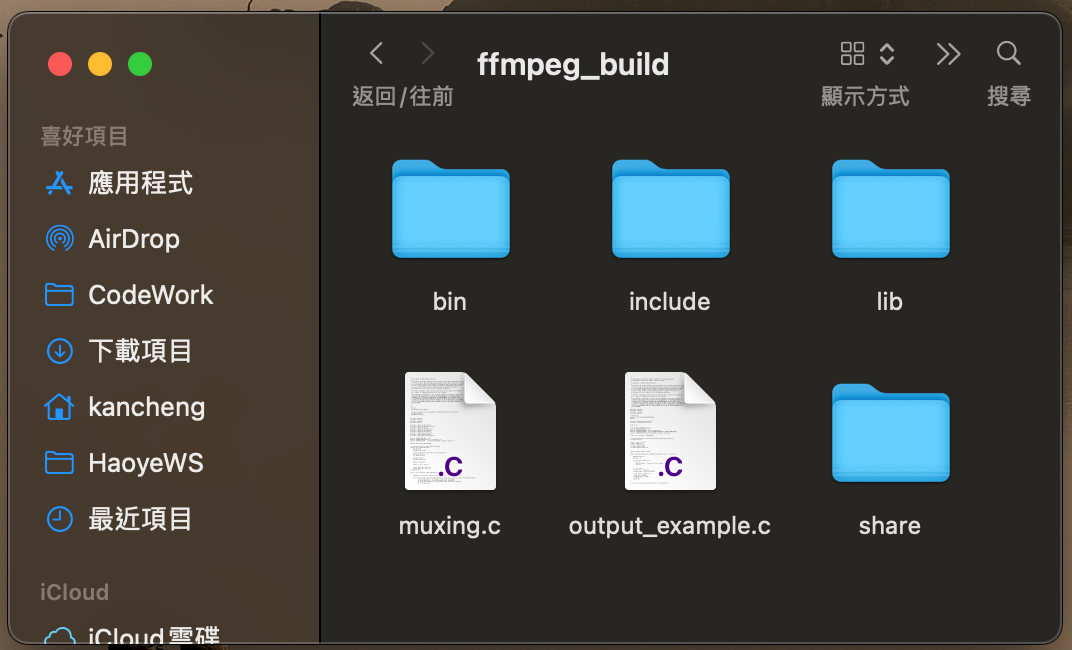
\includegraphics[width=0.50\textwidth]{new.png} 
\caption{muxing.c 目錄}
\label{Test}
\end{figure}

\begin{figure}[H]
\centering 

\includegraphics[width=0.50\textwidth]{tem2.png} 
\caption{muxing.c 測試結果}
\label{Test}
\end{figure}


%\section{附錄}

% 數學意義說明

% $$\min \limits_{G}\max \limits_{D}{V_I(D,\ G)=V(D,G)-\lambda L_I(G,Q)}$$

%	\begin{lstlisting}[language={python}]

%	\end{lstlisting}

%\begin{enumerate}
%\item Y
%\item A
%\end{enumerate}

% \newpage

\clearpage

\end{document}